\section{Documents}\label{sec:fa_documents}

\subsection{Variability Requirements}\label{sec:fa_documents_variability_requirements}

The document editor present in \emph{escolinhas.pt} is one of the core components of the system and one of the used features of the platform. This being the case, and due to the constantly evolving nature (\textbf{FIXME: it's not the nature that constantly evolves, but the product}), it is also one of the most modified parts of the system. As it can be seen in Fig.~\ref{fig:documents_current}, this structure has to grow both in size and complexity every time a new type of block content is introduced --- represented by the gray entities in Fig.~\ref{fig:documents_current}. This means that whenever a new type of content is introduced in the system, which happens somewhat frequently --- from three types of blocks (\emph{Paragraphs}, \emph{Drawings} and \emph{ImageDocuments/Photos}) in September 2009 to seven in April/May 2010 --- it is necessary to setup a new \textsc{ActiveRecord} class (along with all the logic for versioning) and a new \textsc{Controller} to accept the requests necessary to create, edit or delete any of these entities. Despite working as intented, this workflow is not adequate to the constant evolution and prototyping the document editor is subjected to.

\begin{figure}[H]
  \centering
  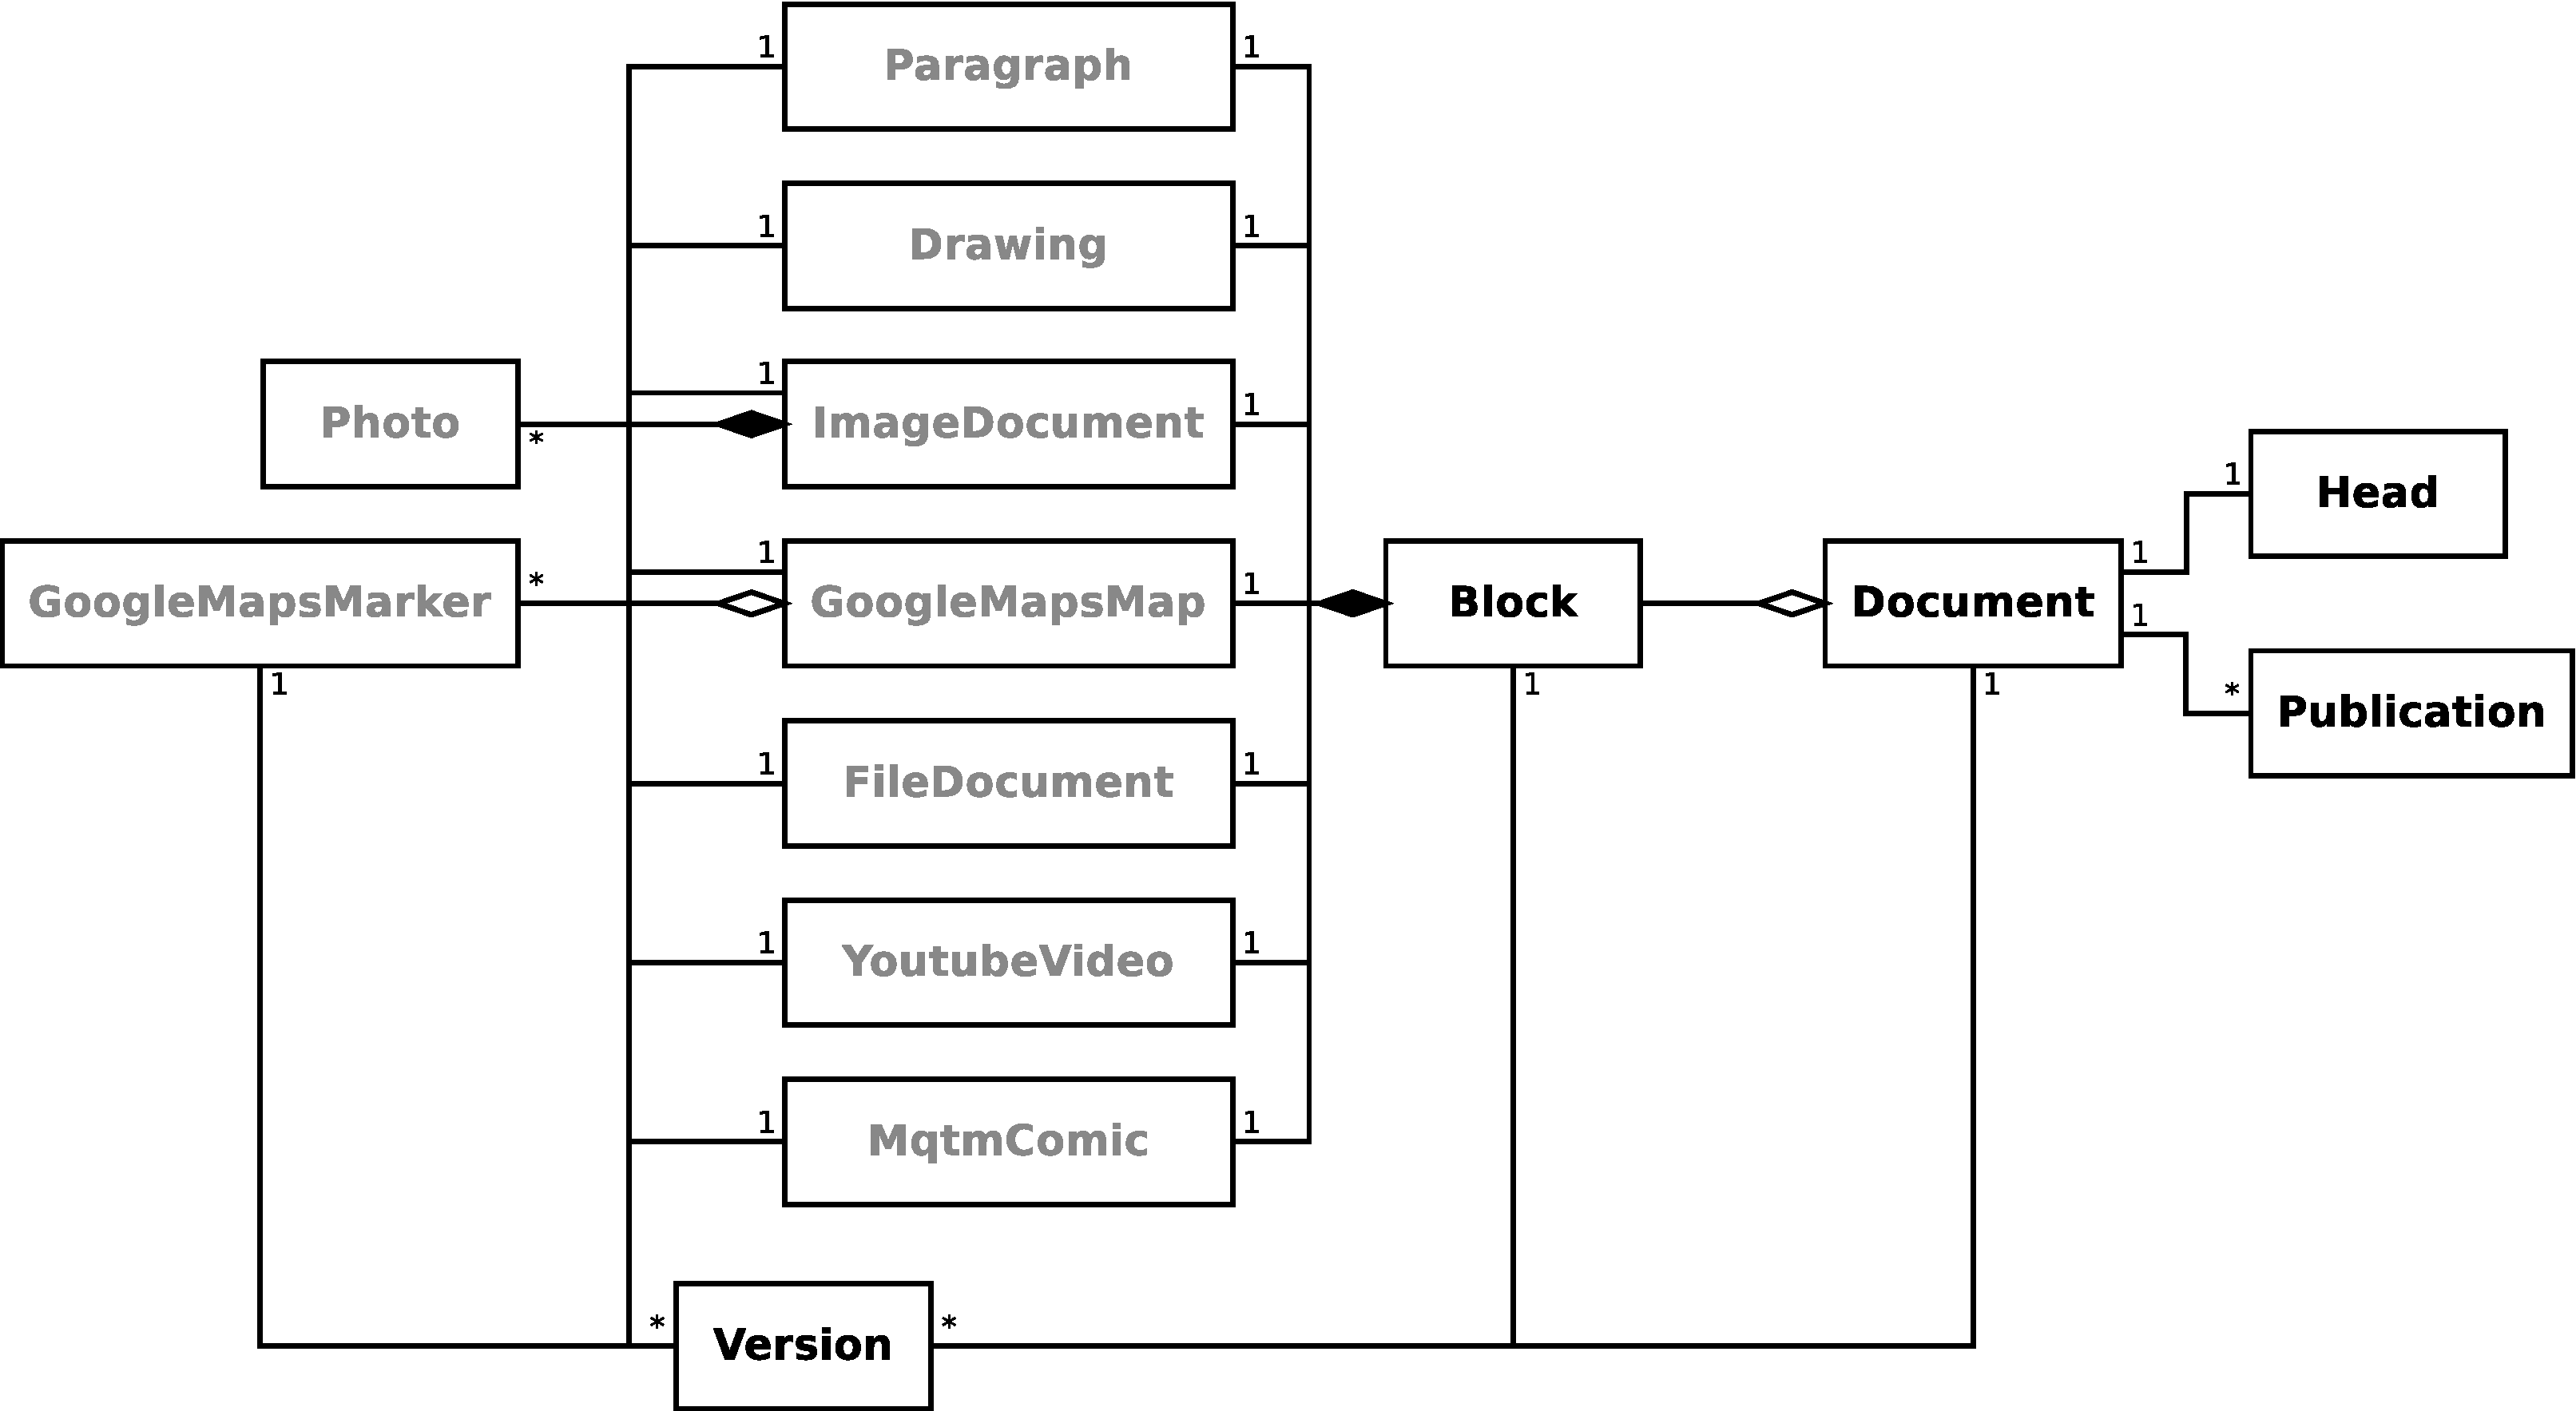
\includegraphics[width=165mm]{documents_current.pdf}
  \caption{Current Documents Model}
  \label{fig:documents_current}
\end{figure}

\subsection{Candidate Patterns}\label{sec:fa_documents_candidate_patterns}

\subsection{Chosen Patterns \& Rationale}\label{sec:fa_documents_chosen_patterns_rationale}

The pattern used is a composite design pattern \cite{riehle_composite_patterns}, where various smaller design patterns work in tandem to create a more complex pattern.

\begin{figure}[H]
  \centering
  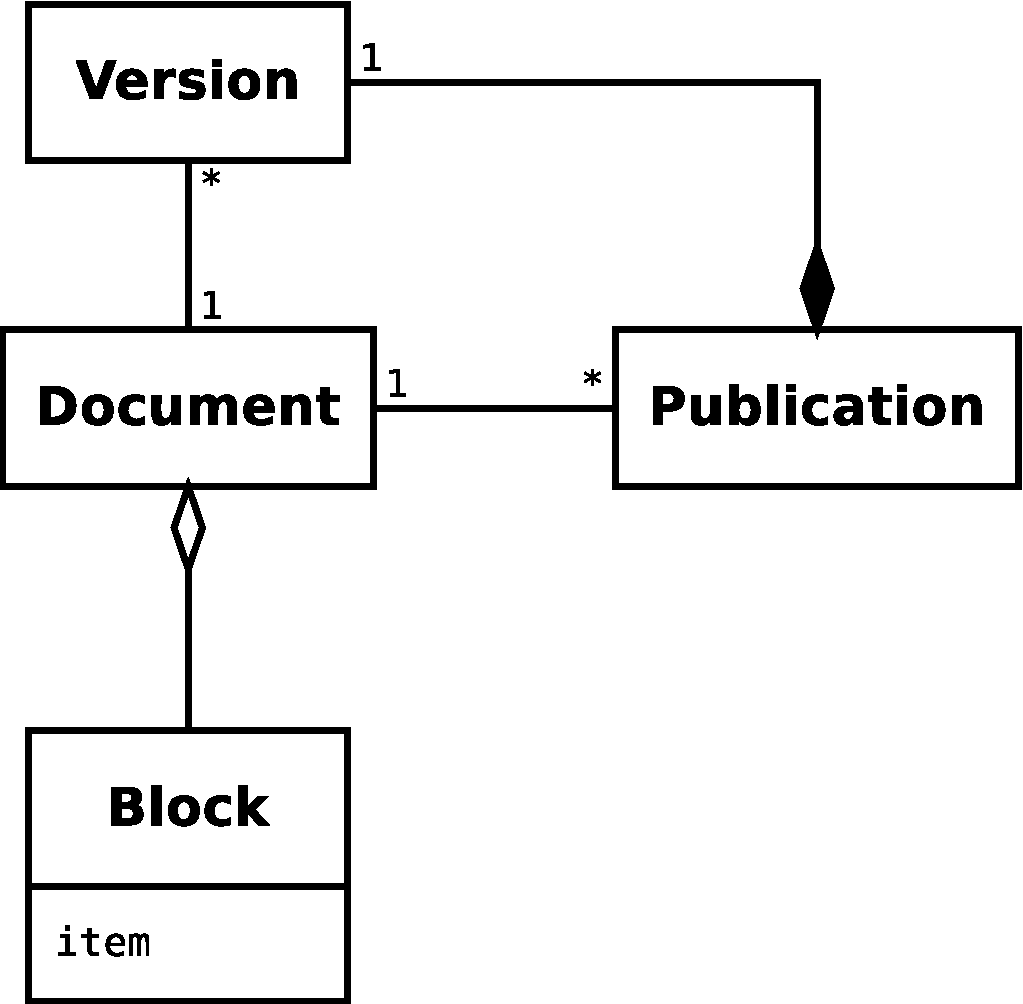
\includegraphics[width=75mm]{documents_conceptual.pdf}
  \caption{Conceptual Documents Model}
  \label{fig:documents_conceptual}
\end{figure}

\textbf{FIXME}

patterns used
\begin{itemize}
  \item \textsc{Memento} - used for versioning
  \item \textsc{Property} (simplified variant) - used for decoupling the type of the block item from the database schema
  \item \textbf{INVESTIGATE: pattern 3} - the fact that a \emph{Publication} points to a specific \emph{Version} of a \emph{Document} may be a pattern --- it works as a \emph{tag} in a VCS (version control system) system such as git or SVN.
\end{itemize}

The variant of the \textsc{Property} pattern implemented is simplified to the highly dynamic nature of the Ruby language --- which means that, for this particular problem, it is able to build new types of objects or even create new class definitions in runtime.

\subsection{Implementation}\label{sec:fa_documents_implementation}

The implementation of this composite pattern takes advantage of the highly dynamic nature of the Ruby language and the API provided by the \textsc{ActiveRecord} implementation of Rails.

\emph{Document}, \emph{Block}, \emph{Version} and \emph{Publication} are all AR objects, which means that, according to the AR pattern and the Rails framework conventions, each one of them is stored inside an SQL table, with a row for each one of the attributes. This structure provides the basic blueprint (as stated in \ref{sec:case-study_areas_document_editor}) for the documents to be produced by the editor --- it allows a title, an arbitrary number of orderable blocks, and a snapshot (version) of each modification. It also allows for publications, which essentially point to a specific version of a document.

There is nothing really remarkable about \emph{Blocks}, \emph{Documents} of even \emph{Publications} --- they are ordinary \textsc{ActiveRecord} objects, with associations to eachother (as pictured in Fig.~\ref{fig:documents_conceptual}), and explaining how they work is outside of the scope of this study.

\emph{Versions}, and \emph{Blocks} content, on the other hand, have special ?features? that, together with AR, are able to provide a truly dynamic and variable staple for the development of document.

As a \emph{Block} is simply a generic container for an arbitrary type of content, a \emph{Block} content can't be constrained to a single class or object type. The solution is to serialize the content inside the \emph{content} attribute of a \emph{Block}. This way, a \emph{Block} content is simply a string that represents a serialized object --- which can be de-serialized, accessed and modified at runtime. This means that, whichever a \emph{Block} content may be, the content itself is responsible for its representation and life cycle.

\subsection{Impact Analysis}\label{sec:fa_documents_impact_analysis}











